\section{Policies}
\subsection{Base Model}
	Before the policies for addressing the problem are presented, it is necessary to show that, indeed, there is a problem and that it can be seen in the model constructed. For this, the base model will be presented, with results for both price and growth rate.

	The results for the base model test are shown in Figure \ref{img:base}, for both price (a) and growth rate (b).
	\begin{figure}[H]
      \centering
      \begin{subfigure}[t]{0.4\textwidth}
        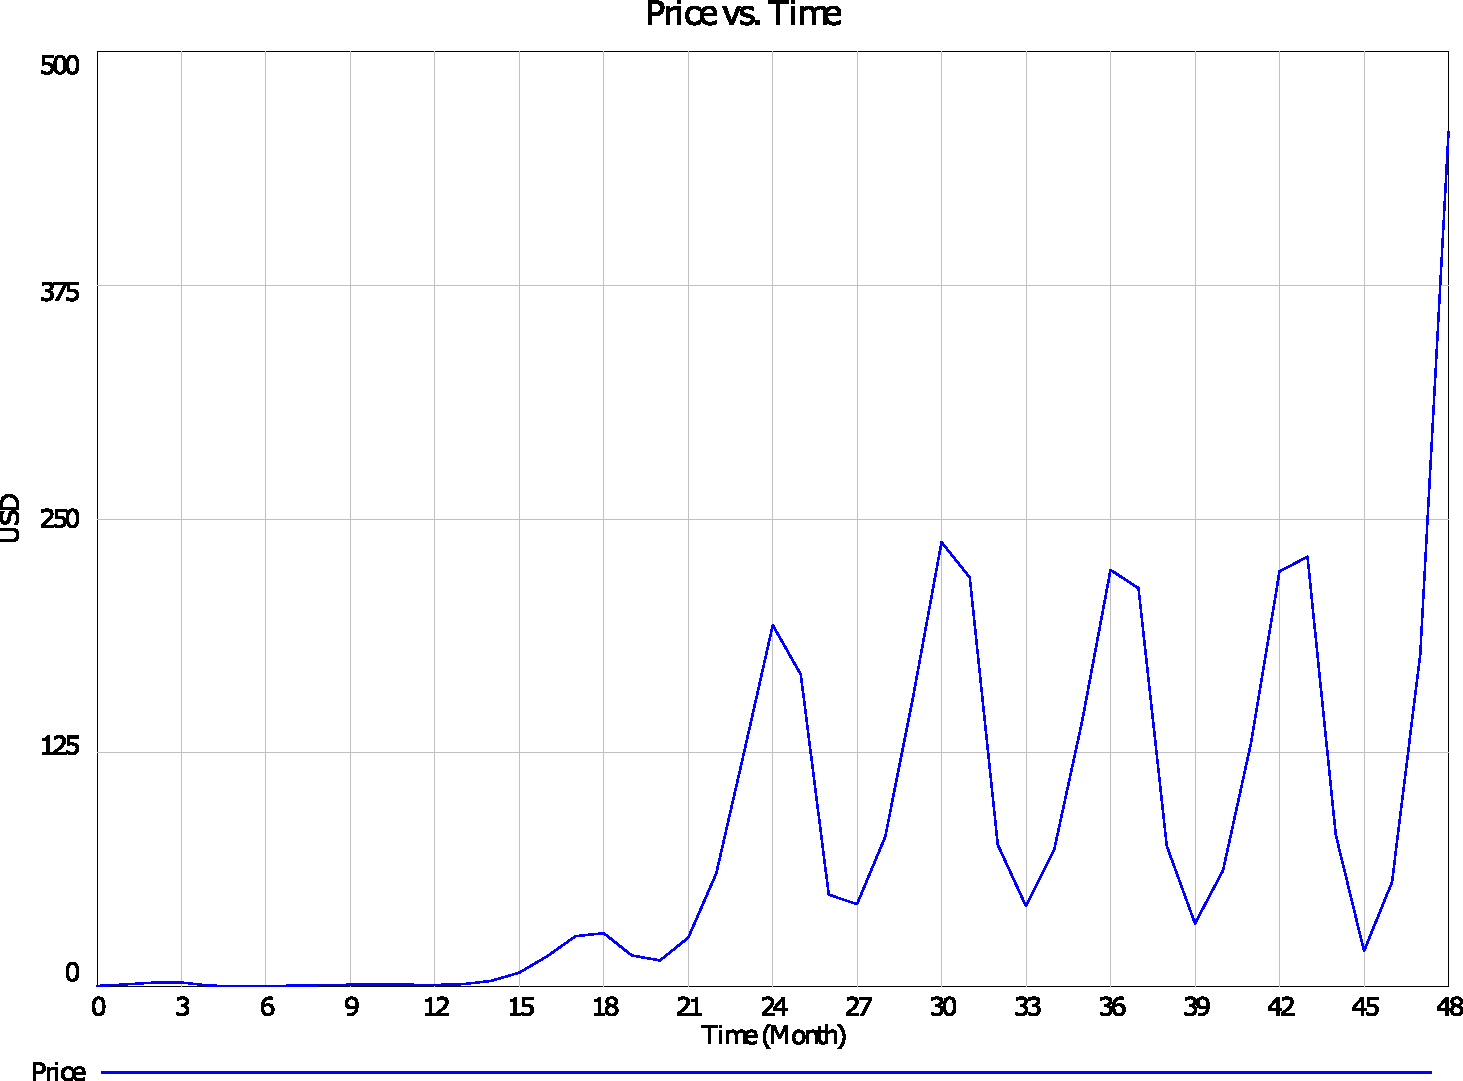
\includegraphics[scale = 0.3]{files/BasePrice.pdf}
        \centering
        \caption{Results for price.}
      \end{subfigure}
      \hspace{1cm}
      \begin{subfigure}[t]{0.4\textwidth}
        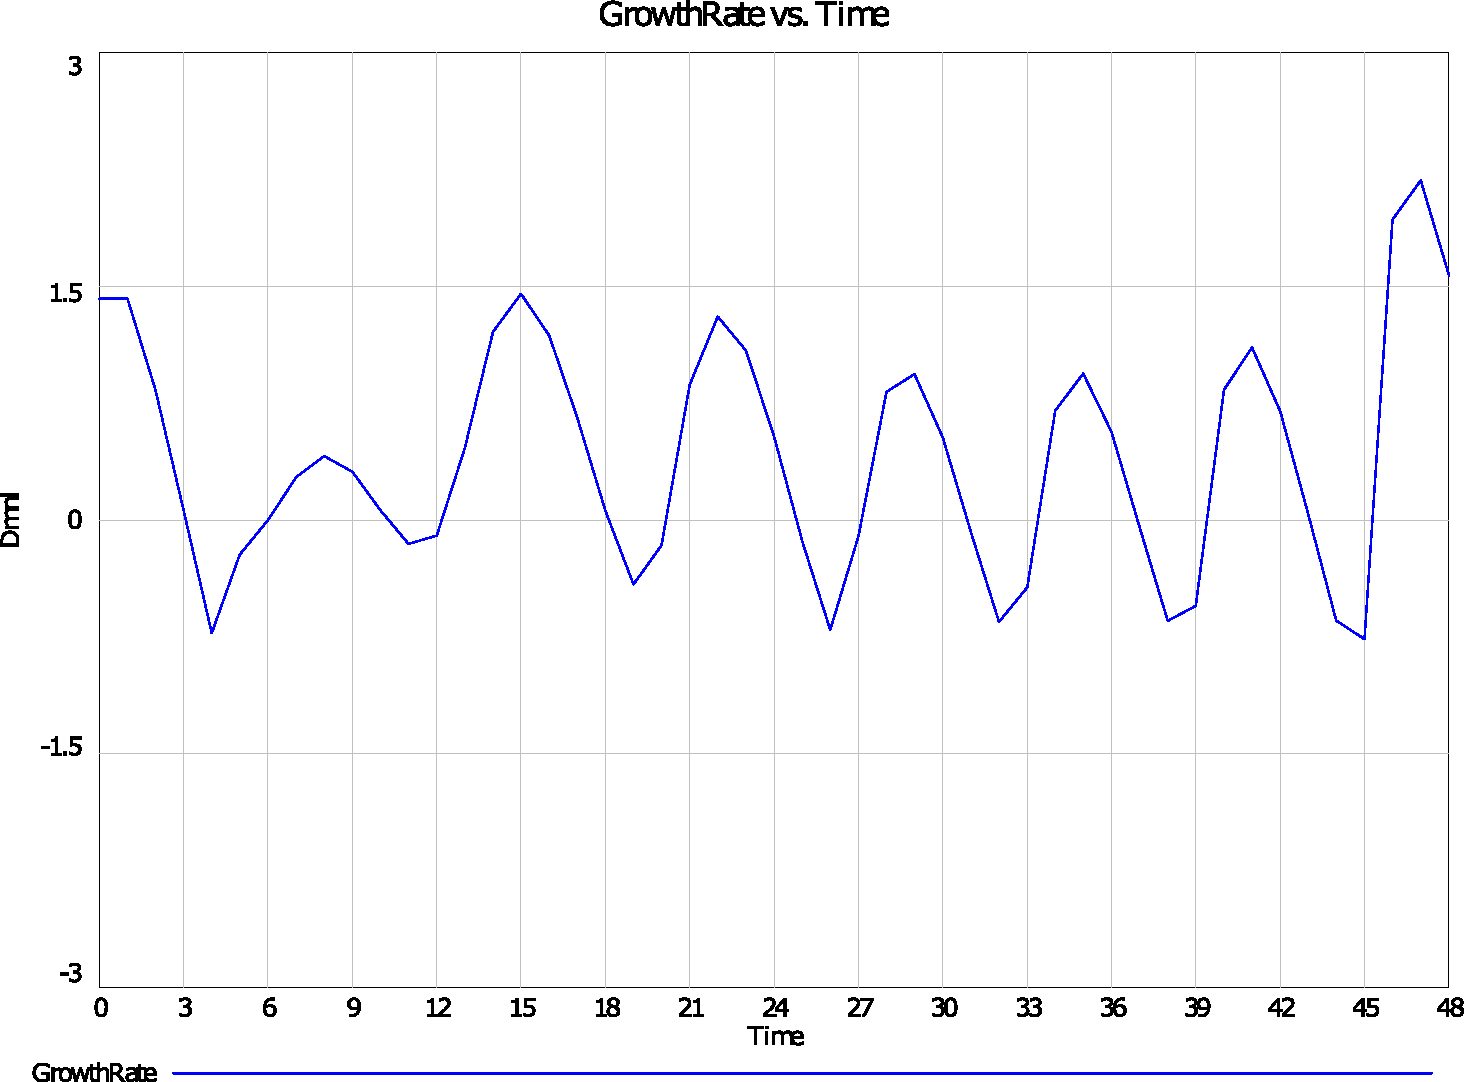
\includegraphics[scale = 0.3]{files/BaseGrowth.pdf}
        \centering
        \caption{Results for growth rate.}
      \end{subfigure}
      \caption{Base model test.}
      \label{img:base}
	\end{figure}
    
   It can be noted that the plot of price (Figure \ref{img:base}.a) for the base model is similar to Figure \ref{img-pricebcc}, which shows price of BitConnect Coin; showing a significant growth in the price of the CC in a very short time period. The problem that is going to be addressed is attempting to limit this growth or, at least, extend the time that the market needs to reach similar prices. A possible improvement to control the system using the model, can be through two specific variables: taxes and investors. 
   
   \subsection{Policies: Government Taxes to Exchanges}
   The first one is controlling the trading in the exchanges, this may be achieved through the government imposing taxes to the exchanges; as the exchanges have to pay to the government, they have to augment their own taxes (exchange fees), so this will represent a change in the price and obviously in the growth rate, as is shown in Figure \ref{img:polittaxes}.
   
   \begin{figure}[H]
      \centering
      \begin{subfigure}[t]{0.4\textwidth}
        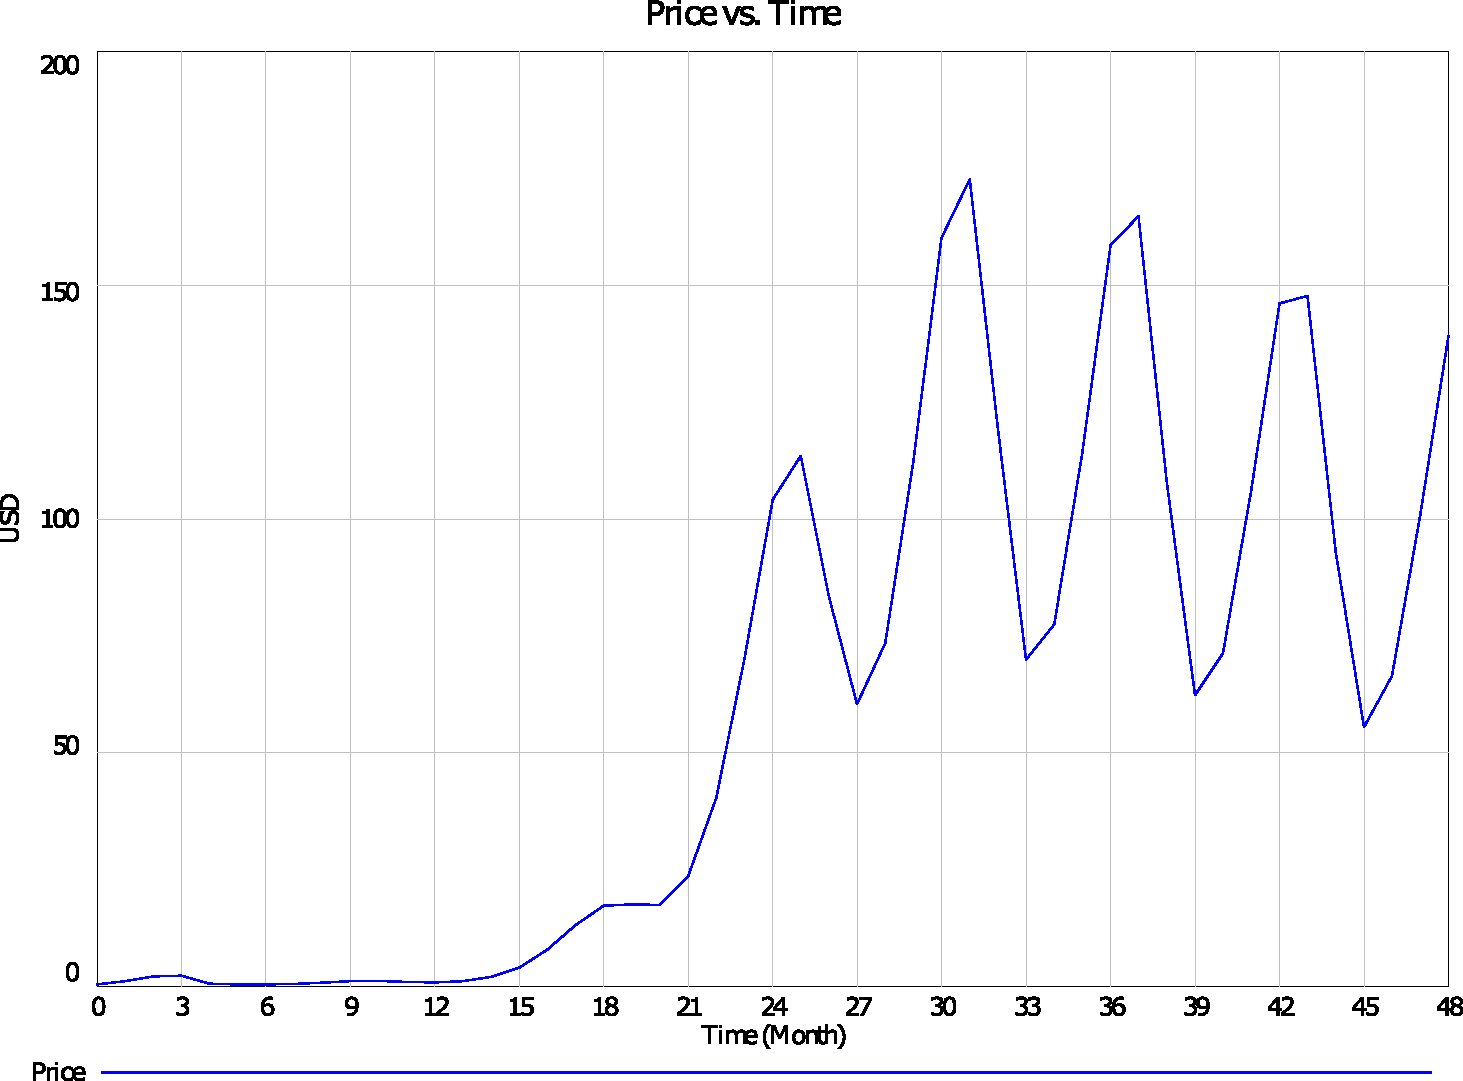
\includegraphics[scale = 0.3]{files/politTaxesPrice.pdf}
        \centering
        \caption{Results for price.}
      \end{subfigure}
      \hspace{1cm}
      \begin{subfigure}[t]{0.4\textwidth}
        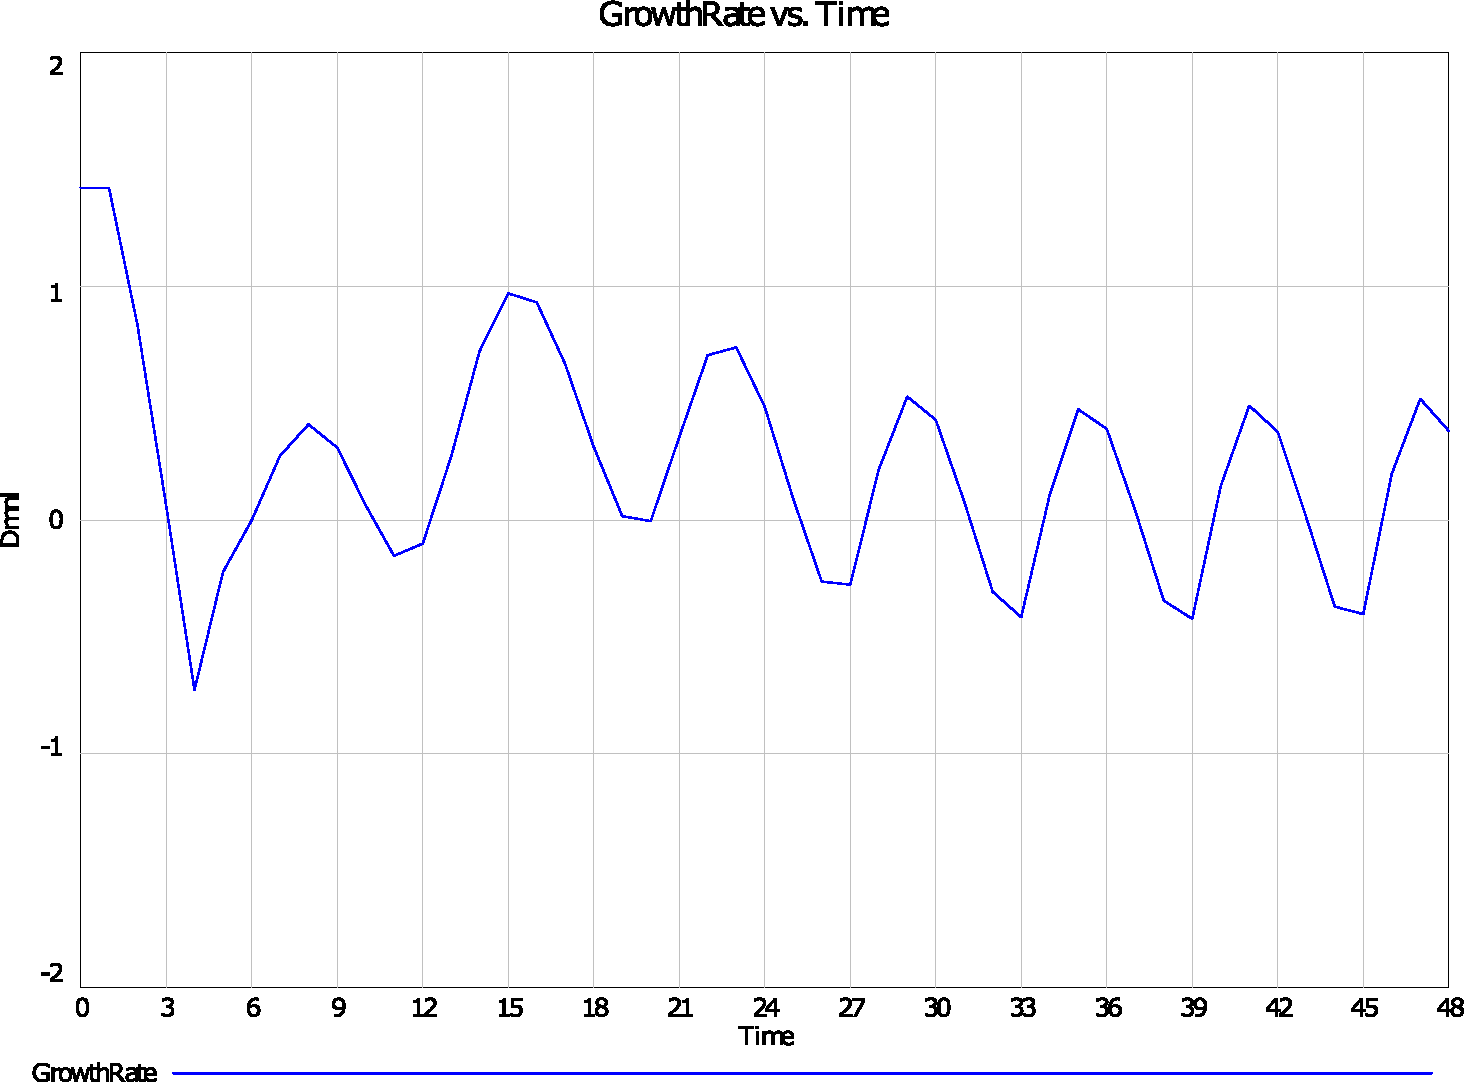
\includegraphics[scale = 0.3]{files/politTaxesGrowth.pdf}
        \centering
        \caption{Results for growth rate.}
      \end{subfigure}
      \caption{Results after setting government taxes.}
      \label{img:polittaxes}
	\end{figure}
   Note that the growth rate keeps a normal fluctuation and that the price is oscillating and tending to drop, as well as the price maximum is around 175USD, whereas the base model was around 480USD; this shows that the policy is effective and changes are taking place in the model results.
   
   
   \subsection{Policies: Limit the Number of New Investors}
   one of the most important factors that rise the price of a cryptocurrency is the number of investors that a certain cryptocurrency can handle a great amount of people. In this order, it is of the utmost importance to regulate the number of  investors that can enter the system monthly so the price grows in a more balanced way. Therefore, we tested the system allowing only ten thousand people maximum to enter the system per month; in the real system, is not that hard to control this aspect but it needs government regulation to make it achievable. The results of this policy can be observed in Figure \ref{img:politinv}
   
    \begin{figure}[H]
      \centering
      \begin{subfigure}[t]{0.4\textwidth}
        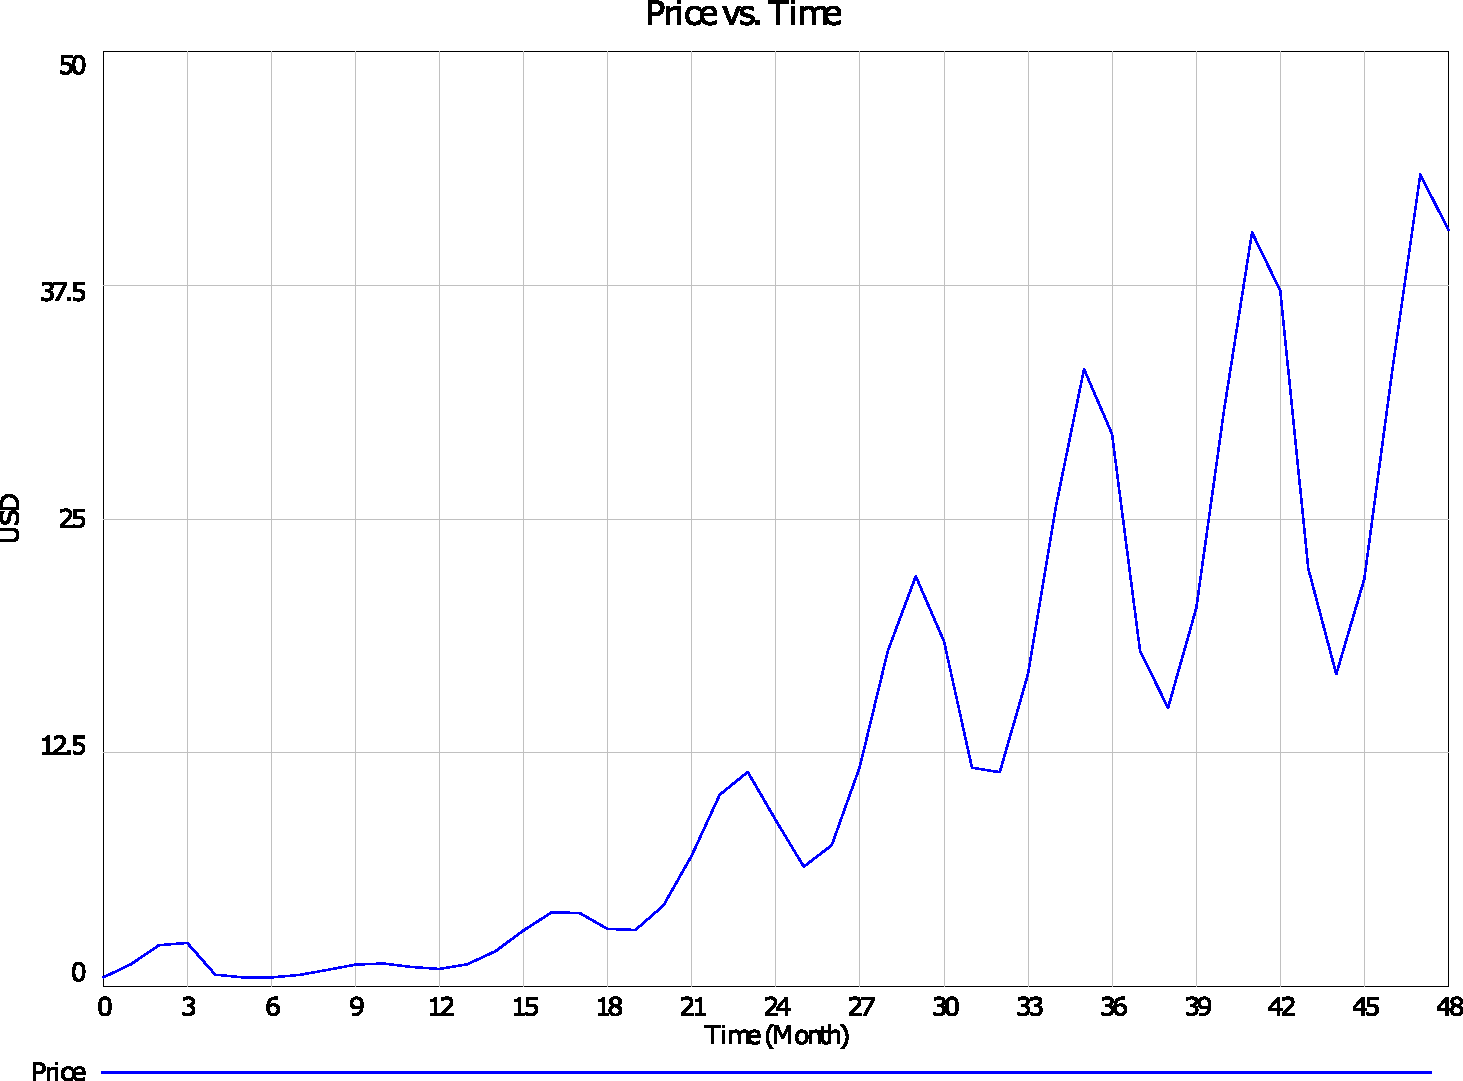
\includegraphics[scale = 0.3]{files/politInvPrice.pdf}
        \centering
        \caption{Results for price.}
      \end{subfigure}
      \hspace{1cm}
      \begin{subfigure}[t]{0.4\textwidth}
        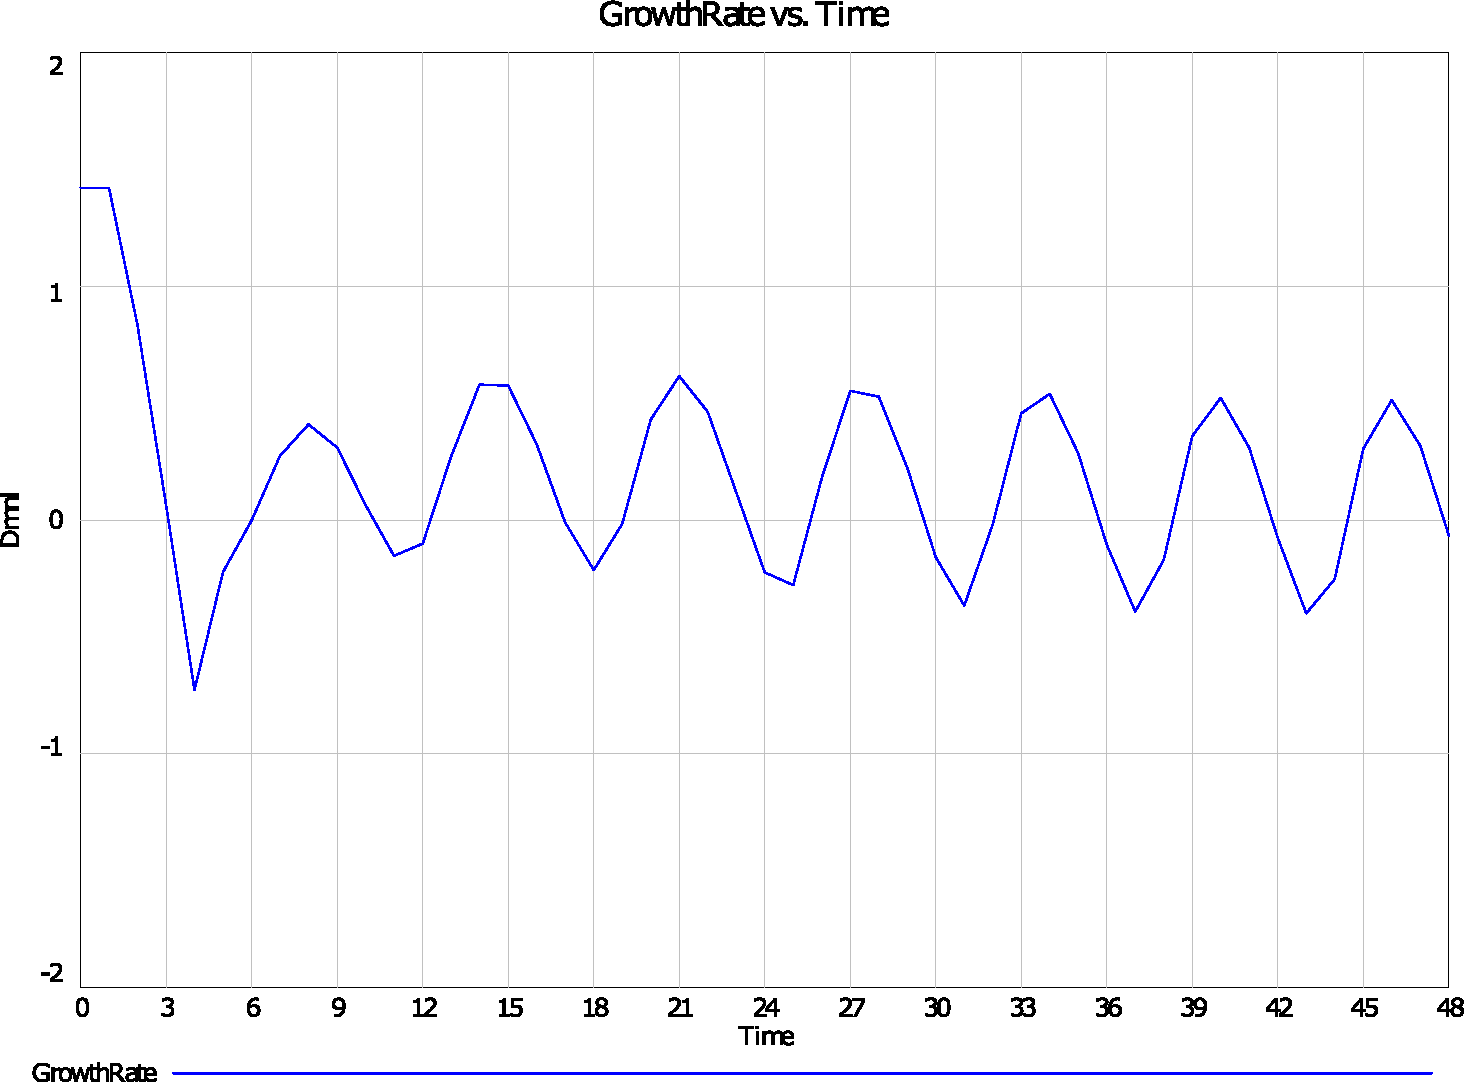
\includegraphics[scale = 0.3]{files/politInvGrowth.pdf}
        \centering
        \caption{Results for growth rate.}
      \end{subfigure}
      \caption{Results after limit in New Investors.}
      \label{img:politinv}
	\end{figure}
